\documentclass[10pt, a4paper, fleqn]{article}

\usepackage{amsmath}
\usepackage{natbib}
\usepackage{graphicx,subfig}
\usepackage[explicit]{titlesec}
\usepackage{appendix}
\usepackage[sc]{mathpazo}
\usepackage{aeguill}
\usepackage[utf8]{inputenc}
\usepackage{soulutf8}
\usepackage{lineno}


\pagestyle{myheadings}
\setlength{\textwidth}{14cm}
\setlength{\mathindent}{1cm}
\setlength{\parindent}{0.5cm}
\setlength{\parskip}{1.5ex}
\setlength{\oddsidemargin}{0.3in}
\setlength{\evensidemargin}{0.6in}
\linespread{1.5}
\setcounter{secnumdepth}{3}
\textfloatsep = 1.5cm
\intextsep = 1 cm

\newcommand{\red}[1]{\textcolor{red}{\st{#1}}}

\newcommand{\focal}{\textrm{f}}
\newcommand{\partner}{N-1}
\newcommand{\z}{z}
\newcommand{\feco}{f_N}
\newcommand{\e}{\beta}
\newcommand{\de}{\mathop{}\! \mathrm{d}}
\newcommand{\s}{S}
\newcommand{\pa}{\pi}
\newcommand{\pav}{\boldsymbol{\pi}}
\newcommand{\br}{b}
\newcommand{\Z}{\mathcal{B}}
\newcommand{\zm}{b}
\newcommand{\ut}{u}




\begin{document}

\title{Cooperation in large-scale human societies -- What, if anything, makes it unique, and how did it evolve?}
\author{Simon T. Powers\thanks{Corresponding author. Address: School of Computing, Edinburgh Napier University, Edinburgh, EH10 5DT, United Kingdom. Email: S.Powers@napier.ac.uk}
\\
Carel P. van Schaik\thanks{Address: Anthropological Institute \& Museum, University of Z\"{u}rich, Z\"{u}rich, Switzerland. Email: vschaik@aim.uzh.ch}
\\
Laurent Lehmann\thanks{Address: Department of Ecology \& Evolution, University of Lausanne, CH-1015 Lausanne, Switzerland. Tel: +41 21 692 4183. Email: Laurent.Lehmann@unil.ch}}
\maketitle
\date{}

\newpage
\linenumbers 
\begin{abstract}

There is much controversy about whether the cooperation underlying the functioning of human societies is explained by self-interest. Confusion over this has frustrated the understanding of how large-scale societies could ever have arisen and been maintained. To clarify this situation, two questions need to be distinguished and answered. First, how exactly do individual cooperative interactions in small- and large-scale societies differ? Second, are the decision-making mechanisms used by individuals incentive driven or incentive incompatible, and are they domain-general or specific to ancestral social environments? We address these questions by reviewing the literature on cooperation across societal scales and the literature on hypothesised decision-making mechanisms. This allows us to delineate between the cultural group selection and institutional-path hypotheses for explaining the origin of large-scale cooperative societies. The former appears incompatible with much of evolutionary biology and social science, while the latter is compatible and provides a parsimonious explanation based on self-interest.
 
\end{abstract}

\noindent Keywords: human social evolution, large-scale societies, cooperation, evolutionary psychology, cultural group selection, institutions 

\newpage

\section*{Introduction}

Understanding how large-scale human societies arose and function is a fundamental question in science. It raises the question of how far this can be explained by the self-interested actor model common to the fields of (political) economics \citep{MasCollelWG95,PindyckR01,Ober:2008:a,Fukuyama:2011:a}, archaeology \citep{Stanish:2017:a} and evolutionary biology \citep{Alexander:1990:a,Parker:1990:a,Davies:2012:a,Alcock:2013:a}. And it is crucial to improving our ability to engineer solutions to societal challenges, including climate change \citep{Milinski:2008:a,Tavoni:2011:a}.

The fundamental social behaviours that allow human societies to function are cooperative, as exemplified by exchange of resources between individuals and contribution to collective-action projects. Unlike any other species, humans today rely on exchange of resources with non-kin for nearly all of their vital needs, from food, to shelter, to medical care. Individuals exchanging resources are often unrelated and unfamiliar strangers, who know little if anything about each other and engage in massively large-scale and spatially-distributed collective-action projects. The contrast between modern human social behaviour and that of other social species is exemplified by the existence of the international space station -- a pinnacle of human cooperation \citep{Turchin:2015:b}. Constructing the space station required contributions of millions of taxpayers from multiple states, and required approximately three million person-years to build. It also involved massive division-of-labour and specialisation in the production of its component parts. 

The human species has spent most of its existence living in small-scale hunter-gatherer societies \citep{Boehm:1999:a,Marlowe:2005:a,Kelly:2013:a}. There is much cooperation in these societies, from food sharing, through to cooperative hunting and construction of dams \citep{Kaplan:2009:a,Jaeggi:2013:a,Hooper:2015:a}. But this cooperation occurs in small groups where individuals are either kin or personally know each other, directly or indirectly by reputation. Following the origin of agriculture around 10000 years ago, humans started to live in larger and larger groups, culminating in the modern states and space stations of today. These larger groups are only viable because of exchange and collective-action occurring between individuals. But why would individuals cooperate in this new environment? Do the same evolutionary processes that selected for cooperative behaviour in small-scale societies, and other primates, provide a sufficient explanation \citep{Alexander:1987:a,Cosmides:1992:a,West:2011:a,Tooby:2016:a} or is \textbf{a different} evolutionary process needed \citep{Richerson:2005:a,Turchin:2015:b,Henrich:2016:b}? Can cooperation in large-scale societies be equilibrium behaviour among self-interested individuals \textbf{that act to  maximise their own individual benefit \citep{North:1990:a,Greif:2006:a,Powers:2016:a}}, or are individuals no longer be acting in their own \textbf{private} self-interests \citep{Richerson:2005:a,Bowles:2011:b,Turchin:2015:b,Henrich:2016:b}?

Despite much debate, there has been little movement towards a consensus on these questions, and hence little scientific progress in understanding the transition from cooperation in small-scale societies to that in large-scale societies. To resolve this impasse, \textbf{three factors need to be disentangled qualitatively and resolved quantitatively. First, what are social interactions within large-scale societies like? Are they qualitatively different from those in small-scale societies (involving fundamentally new kinds of interactions), or is the scaling up of interactions merely quantitative?  Second, there is a need to determine the evolved decision-making mechanisms used by individuals in social interactions. To what extent is decision-making incentive driven? And is it domain-general, or is it specific to the types of social situation encountered in ancestral environments? Because the decision-making mechanisms are likely to be complex cognitive traits with a genetic basis, they are unlikely to have changed significantly during the few thousand years since the origin of large-scale societies. This means that the same evolved decision-making mechanisms must be used by individuals in both small- and large-scale societies. Finally, how are behaviours transmitted between individuals within and across generations? Does transmission of behaviour mainly involve individuals imitating those in their group or other groups, or is the physical movement of individuals between groups (e.g. through warfare or migration) more important? Resolving these three factors narrows down the space of possible hypotheses purporting to explain the transition in cooperation from small- to large-scale societies.} 

%two factors need to be disentangled qualitatively and resolved quantitatively. First, there is a need to establish whether cooperation in large-scale societies is different (involving fundamentally new kinds of interactions) from that occurring in small-scale societies, or is just a scaled-up version of the same problems that hunter-gatherers faced. Second, and regardless of the scale of society, there is a need to determine the decision-making mechanisms used by individuals in social interactions. Potential decision-making mechanisms need to be separated along two dimensions. First, is behaviour incentive-driven by payoff, or do individuals copy others regardless of payoff incentives? Second, is behaviour the outcome of a domain-general information processing mechanism, or is it domain-specific to the types of social situation encountered in ancestral environments? Answering these questions is central to characterising the type of interactions individuals experience in large-scale societies, what broad type of agents (or``mind'') they are, and what constraints this places on action choice. This, in turn, narrows down the space of possible hypotheses purporting to explain the transition in cooperation from small- to large-scale societies.

\textbf{In this paper, we address this by synthesising what the empirical literature tells us about the similarities and differences between social interactions across societal scales, and what it tells us about the decision-making mechanisms used by individuals. We also consider different ways by which behaviours are transmitted between individuals. We then combine these three elements to show the explanations that they entail for the transition from small- to large-scale societies.}

\section*{How are social interactions different in small- and large-scale societies?}

In evolutionary biology an individual's actions tend to be defined as cooperative if they increase the lifetime survival and/or reproduction of both the actor and recipient(s) \citep{Axelrod:1981:a,Rousset:2004:a,lehmannKellerFramework,Bshary07}. We follow this definition here but always consider cooperative behaviours that involve a social dilemma \citep{Kollock:1998:a}, which is a situation where a material payoff to other group members is increased by an action that is ``costly" to an individual compared with not doing the action, in the sense that it decreases the actor's share of the group's material payoff \citep{Dawes:1980:a}. Material consequences of actions are usually multidimensional, e.g. calorie intake, size of shelter, or time of activity. But we can assume that all material consequences of behaviours can be summarised by a single number, the material payoff to an individual, from which group material payoff can also be evaluated. \textbf{Material payoff is therefore a unifying currency across evolutionary biology, behavioural ecology and economics}. \textbf{Self-interested individuals act as if to maximise their expected lifetime material payoff}.

For more than 2 million years nomadic hunter-gatherers lived in small-scale societies. Following sedentarisation and the subsequent Neolithic Demographic Transition around 10 000 years ago \citep{Bocquet-Appel:2011:a}, large-scale societies arose. These societies are large in terms of number of individuals, and tend to have hierarchical organisation, i.e. chiefdoms and states \citep{Johnson:2000:a}. To discuss the differences and similarities of cooperation in small- and large-scale societies, we start by introducing a model of social interaction that underpins our analysis and that is independent of societal scale. 



\subsection*{Cooperation in terms of material outcomes}

We take our model of social interaction from game theory \citep{Fudenberg:1991:a,Hurwicz:1996:a}, as this provides a common reference model across the biological and social sciences \citep{Gintis:2007:a}. We consider that a social interaction consists of the behaviours (actions or stream of actions) of individuals and the outcome(s) of such behaviours, measured in terms of material payoff. The set of possible social interactions is formally called a \textit{game form} \citep{Hurwicz:1996:a,Fudenberg:1991:a}. This defines the behavioural options —- the strategies (e.g. cooperate or defect)  —- available to individuals, and their material outcomes. Colloquially, a game form specifies the ``rules of the game'' or simply the ``game'', a shorthand often used in evolutionary biology that we use here.

A key observation of human social interactions is that individuals can change the rules of the game that they play \citep{North:1990:a,Ostrom:1990:a,Hurwicz:1996:a,Greif:2006:a,Kaplan:2005:a}. An \textit{institution} is defined as a family of games (game forms) that individuals can potentially choose between, given the current state of the physical environment and their technology \citep{Hurwicz:1996:a}. The hallmark of an institution is the presence of two sets of social interactions
\citep[p.~3]{Powers:2016:a}: (i) active genesis of institutional rules through communication and/or bargaining by the individuals in a group -- this is the political game \citep{Hurwicz:1996:a,Reiter:1996:a}; (ii) social interactions whose outcomes are material and which are affected by the institutional rules -- this is the economic game. The key idea behind an institution is the formalisation of the point that humans, unlike other animals, can self-modify the material payoff structure of their social interactions. They thus play both political and economic games, where the former generates the institutional rules defining the latter. 

\subsection*{Two types of cooperation}

Any cooperative act in the economic game can be placed on a scale representing the excludability of the economic good that it involves. At the one end of this scale is the voluntary exchange of private goods between individuals. These are goods that the actor controls or otherwise has property rights over, meaning that other individuals can readily be excluded from using them. Exchange of private goods can be mutually beneficial by allowing individuals to obtain resources that they want but do not currently have. It also allows gains in efficiency from division of labour and specialisation \citep{North:1990:a,Greif:2006:a}. But it is not obvious that individuals will choose to engage in exchange, for two reasons. First, one individual must part with its goods before it receives anything in return. This means that an individual risks being cheated and receiving nothing in return \citep{Greif:2000:a}. Second, the individual offering a good inherently knows more about its quality than the receiver, creating an information asymmetry that can be used to exploit the other party \citep{North:1990:a}. Hence, exchange involves a social dilemma. 

At the other end of the excludability scale are collective actions that involve the production and consumption of public goods such as village fortifications, or common-pool resources such as fish stocks, grazing land, or irrigation water \citep{Hardin:1968:a,Ostrom:1990:a}. It is costly to monitor the behaviour of individuals producing and using this type of good, and hence to exclude those that do not contribute. This means that there is a social dilemma because of the temptation to enjoy the benefits without cooperating in their production \citep{Olson:1965:a}. 

In the following discussion we categorise cooperative acts based upon whether they are closer to private (exchange) or public goods/common-pool resources (collective action) on the excludability scale. 

\subsection*{The world until yesterday: Cooperation in small-scale societies}

\subsubsection*{Exchange}

Hunter-gatherers engage in several types of exchange. The most well studied is the exchange of meat between large-game hunters, i.e. food sharing. Male hunters donate food to other hunters in their group when they make a kill, and in turn receive food when the latter are successful. The exchange occurs repeatedly -- essentially for an indefinite number of times -- between members of the camp, which would number around 30 individuals \citep{Marlowe:2005:a,Kelly:2013:a}. The exchange is also personal \citep{North:1990:a,Greif:2006:a}. People obtain first-hand information about the behaviour of others -- they remember exactly who they have given food to in the past, and remind them of this when they are themselves hungry. This is supported by systems of institutional rules that regulate the conditions under which individuals should give food to others, and which apply to the whole group \citep{Kaplan:2009:a}. Group members enforce these rules upon each other through a variety of sanctions ranging from gossip and public ridicule through to hiding and ostracism \citep{Boehm:1999:a}. Hunter-gatherers also exchange one type of commodity for another. A sexual division-of-labour is evident, particularly between males that specialise in hunting, and females that specialise in gathering plant materials \citep{Marlowe:2007:a}. Among horticulturalists, we see the exchange of horticultural produce for meat, and the exchange of childcare for labour and sick care \citep{Jaeggi:2016:a}.

\subsubsection*{Collective action}

Hunter-gatherers engage in a variety of collective-actions related to subsistence. A prime case is cooperative hunting, where the actions of several individuals are necessary to prevent a prey from escaping \citep{Kaplan:2009:a,Alvard:2002:a}. Hunter-gatherers also engage in various collective construction projects, such as burning habitat, and building dams to trap fish \citep{Kaplan:2009:a}. Because the number of individuals taking part in the collective-action is relatively small, the benefits are immediately and directly felt by the participants. In a small group of five hunters, if one individual does not pull its weight then it will directly feel the impact through a markedly reduced probability of catching prey. The benefits to an individual of cooperating are also returned with a small time delay, e.g. on the order of hours for cooperative hunting, or a few weeks for the construction of dams. The cost that an individual pays to receive this benefit is measured in terms of the opportunity cost of time and labour invested, or the direct contribution of material resources. Institutional rules regulate how exactly the benefits of collective action are distributed. For example, in the !Kung Bushmen, the owner of the first arrow that penetrates the animal controls distribution after a cooperative hunt \citep{Testart:1987:a}.


\subsection*{The world today: Cooperation in large-scale societies}

\subsubsection*{Exchange}

In larger-scale societies we see the specialisation and division-of-labour that already existed in hunter-gatherer societies become much more pronounced. Individuals now specialise in one occupation, and obtain all of their vital resources through exchange with others. And this exchange is impersonal -- it is often with unfamiliar strangers who may never meet again \citep{North:1990:a,Greif:2006:a,Seabright:2010:a}. Consequently, individuals will not have first-hand information about how their exchange partners have behaved in the past. But crucially, the institutional rules of the (economic) exchange game have changed to account for this \citep{Milgrom:1990:a,Greif:1994:a,Greif:2006:a}. For example, credit reference agencies supply information about the reputation of participants who will never physically meet. This is essentially an elaboration of the spreading of reputation by gossip seen in hunter-gatherers. Similarly, the state provides third-party enforcement of contracts through the sanctioning of individuals that do not act according to the agreed terms of an exchange. This acts as an elaboration of the enforcement of exchange norms seen in hunter-gatherer groups. 


\subsubsection*{Collective action}

Large-scale societies also engage in numerous in collective actions, from building roads and fortifications through to the use of irrigation systems and fishing waters. These goods are produced and used by many more individuals, which means that the effect that any one individual feels as a result of its own effort will be negligible.  The result of the collective-action can be delayed by a very long time, often on the order of years. As such, there would seem to be more temptation to not cooperate than in small-scale societies. But crucially, the institutional rules regulating collective actions have also changed. These now include third-party sanctioning by the state, which is facilitated by collecting contributions from taxes whose payment can be easily monitored. New institutional rules also incentivise individuals to monitor each other's use of common pool resources. An example is allowing monitors to keep a share of the fine levied on any individual that they find taking more than the agreed amount of resource \citep{Ostrom:1990:a,Guala:2012:a}.


\subsection*{Comparing cooperation across scales}

As we move from small- to large-scale societies, a change in societal structure must occur to account for the change in size \citep{Bonner:2011:a}. A much higher degree of specialisation and division-of-labour is observed in large societies, a feature predicted by the size-complexity rule: bigger entities have greater division of labour \citep{Bonner:2004:a,Bourke:2011:a}. At the same time, the exchange upon which this division of labour depends becomes more impersonal, with individuals less likely to have first-hand knowledge about the past behaviour of their exchange partners. And in collective action, we see the number of participants become so large that the marginal effect of any one individual's contribution is negligible. 

Qualitatively, though, both small- and large-scale societies face the same types of exchange and collective action problems. The organisational problems just become more difficult in large-scale societies, and as we increase scale we see more institutional rules that spread out into new domains such as long distance trade and large-scale construction projects. The increase in the number of rules with the scale of a society is striking. For example, the small-scale Kapauku Papuan society has around 120 rules regulating areas from property rights through to punishment for murder, whereas 40 000 new laws took effect in the United States in 2014 alone \citep{Singh:2017:a}. From this we can infer that as societies of any scale engage in new economic activities, the number of institutional rules that the society has increases.

\section*{Maintenance of cooperation in societies of any scale}

\subsection*{Three decision-making mechanisms (``agents'')}
%Move discussions about types of social learning, e.g. payoff-biased to the transmission section?
So far, we described the (economic) games individuals play in small- and large-scale societies, and how these are at least in part humanly devised. But in itself this description does not specify how or why individuals take actions.

We now present three main decision-making mechanisms (types of agent) that have been proposed \textbf{in different sub-fields of the literature} to explain how individuals choose actions. \textbf{These agent types are necessarily abstract caricatures of human cognition, since they correspond to the general theoretical assumptions that researchers in different sub-fields make about how human agents choose actions. But while few, if any, researchers would argue that human minds literally function as the agent types presented below, these caricatures are widely used in theoretical models and hence are used to make predictions about how humans will behave. It is therefore necessary to clearly state what assumptions they make about how human actors choose actions} 

We stress that the agent types below are \textit{independent} of the scale of the society, and so apply to explaining behaviour in both small- and large-scale societies. For each hypothesised agent type we indicate what assumptions it makes about how individuals take actions, what type of games it supposes that individuals engage in, and the conditions that must hold for cooperation to be stable given this agent type. We categorise the decision-making mechanisms based on whether they are domain-general, or domain-specific to cooperation, and on whether choice of action is sensitive to expected payoff. 


 
 \renewcommand{\labelenumi}{(\arabic{enumi})}
 \begin{enumerate}
 
 \item \textbf{The Rational Strategising Mind (hereafter RSM).} Individuals are assumed to try to maximize their personal material payoff \citep{MasCollelWG95,Ober:2008:a,Fukuyama:2011:a}. For a behaviour to be expressed it must be a Nash equilibrium of the game at hand and hence incentive compatible \citep{Kreps:1988:a,Hurwicz:1996:a,Fudenberg:1991:a}. \textbf{This is the standard model of human cognition assumed in economics, where it is used to make predictions about how individuals will behave in exchange and collective action situations}. An RSM agent is flexible; it is a \textit{domain-general} and \textit{payoff-sensitive} information-processing behavioural mechanism. There is a whole spectrum of RSMs, from myopic agents choosing actions that maximise short-term payoff, through to fully forward-looking agents that act to maximise long-term payoff. RSMs may incorporate information from payoff-biased social learning, where they copy behaviours from others that they perceive to yield a higher material payoff. 
 
For cooperation to be maintained in exchange and collective action games by RSMs, the games must be repeated with known or unknown individuals. Both the conditioning of actions on past behaviour and enforcement of property rights and contracts by the state can create incentives for this agent to cooperate in large-scale societies.  

 
\item \textbf{The Pleistocene Adapted Mind (hereafter PAM).} Individuals are assumed to express behavioural rules maximising on average their inclusive fitness in the Pleistocene social environment of small-scale societies and personal interactions (the Environment of Evolutionary Adaptedness, or EEA) \citep{Alexander:1990:a,Barkow:1992:a,Cosmides:2013:a}. Human psychology is thus supposed to solve the survival and reproductive puzzles posed by the EEA, and is incentive compatible with the material payoffs obtained in that environment. This is achieved by evolved \textit{domain-specific} behavioural algorithms that were \textit{payoff-sensitive} in the EEA. These are often called modules in evolutionary psychology, and are functionally specialised to solve particular adaptive problems, e.g. language acquisition, mate selection, or cooperative exchange \citep{Lumsden:1981:a,Alexander:1990:a} \citep[p.~24]{Barkow:1992:a}. Modules may do varying amounts of computation, ranging from a complex assessment down to the use of simple heuristic rules (e.g. \citealt{Gigerenzer:2009:a}). \textbf{This is the model of human cognition used in evolutionary psychology, which uses experiments  to try to reconstruct what the modules look like. These reconstructed modules are then used to make predictions about how individuals will behave, based on the selective pressures of the EEA that produced them\citep{Cosmides:1994:a}.} 

%Under this agent type, learning is an overarching mechanism that then allows the particular domain-specific algorithms to deal with phylogenetically novel situations \citepp[p.~259-263]{Alexander:1990:a}, e.g. by setting their parameters \citepp{Hagen:2006:a}. 

The EEA would have selected for a psychology that initiates and monitors reciprocal exchanges, including specialised algorithms for detecting cheaters and calculating the probability that an exchange partner will reciprocate \citep{Cosmides:1992:a}. PAMs would now cooperate in large-scale societies whenever these algorithms were activated with inputs that resembled situations where it would have been incentive compatible to cooperate in the EEA.


\item \textbf{The Biased Imitating Mind (hereafter BIM).} Individuals are assumed to acquire their behaviour mostly from others through forms of biased social learning, in which who else performs the behaviour matters more than the expected material payoff of doing that behaviour \citep{Henrich:2003:a,Richerson:2005:a,Henrich:2016:a}. Conformity-biased learning (copy the behaviour of the majority) or prestige-biased learning (copy the behaviour of a leader) are the main such behavioural mechanisms \citep{Henrich:2001:b,Richerson:2005:a,Boyd:2011:a}. BIMs are \textit{domain-general} but \textit{payoff-insensitive} \citep{Henrich:2004:a}. \textbf{This is the model of human cognition that has been used in theoretical models of cultural group selection \citep{Boyd:1985:a,Henrich:2001:a,Henrich:2004:aa,Andresguzman:2007:a,Boyd:2011:a}, where it is called context-based cultural learning \citep{Henrich:2003:a,Richerson:2005:a}}.  

Because BIM agents are insensitive to material payoff, cooperation could be maintained as an equilibrium behaviour regardless of the (economic) game that they play. This means that how the type of exchange and collective-action games, and hence institutions, incentivise behaviour does not really matter.

\end{enumerate}

\subsubsection*{Comparing the agent types}

\textbf{In reality human cognition will be some mix of the three agent types. However, different models assume that humans are most like one particular agent type. To evaluate how well these models can explain human cooperation, we therefore need to look at the weight of evidence that pulls humans towards and away from each of the agent types.}

To start, note that all three agent types assume that individual behaviour is plastic: none suggest that individuals have a hard-wired response to always cooperate or defect. Further, they all assume that individuals can express behaviour that they learn over their lifetime. 

Figure 1 compares the agent types on the domain-generality scale. This scale separates PAM from the other agent types. Evolutionary psychologists have presented experimental evidence which suggests that humans have some decision-making mechanisms that are domain-specific to cooperation, e.g. for detecting cheaters \citep{Cosmides:2013:a}. However humans, like other mammals, also have some domain-general behavioural processing mechanisms \citep{Burkart:2016:a}. To what extent the decision-making mechanisms that produce human cooperation are domain specific is therefore still an important open question.

Figure 1 also compares the agent types on the payoff-sensitivity scale. PAMs are expected to make incentive compatible decisions in situations that mirror the social environment of the EEA, e.g. where there is information about the past behaviour of potential partners. But they would be expected to undertake incentive-incompatible actions when environmental cues trigger the evolved algorithms in inappropriate circumstances \citep{Johnson:2003:a,Burnham:2005:a,Hagen:2006:a,Raihani:2015:a}. For example, individuals behave differently when ``watched'' by a pair of robotic eyes, which could mistakenly trigger algorithms that are sensitive to reputation \citep{Burnham:2007:a}. BIMs could undertake incentive-incompatible actions whenever other individuals (the majority or the leader) were doing so. RSMs, on the other hand, would be expected to always try to increase their material payoff given the information available to them.

Experimental economics has long demonstrated in the laboratory that individuals are sensitive to material payoffs in exchange games that resemble the types of exchange problems identified above \citep{Smith:1962:a}. Further, the levels of cooperation in a repeated Prisoner's Dilemma experiment are affected by whether the end point of the game is known, implying that individual decisions to cooperate are affected by the equilibria of the game \citep{Roth:1978:a}. Individuals also adjust their behaviour in exchange situations in response to the reputation of their partners \citep{Milinski:2016:a}. This all implies that humans act as if they were RSMs in these situations. 

A different line of research involves experiments where cooperation is not incentive compatible, particularly public goods games without incentives to cooperate, and argues that individuals nevertheless still cooperate \citep{Fehr:2002:b}. This has been suggested as evidence for BIM underpinning ``strong reciprocity'' \citep{Fehr:2002:a,Boyd:2003:a}. However, as in exchange games, when individuals play the game for a longer period of time then they often start to behave in an incentive compatible manner \citep{Binmore:2005:b,Sefton:2007:a}. Further, analysis of multiple experiments reveals that individuals are still responsive to marginal selfish payoffs and that this lowers their contribution levels \citep{Ledyard:1995:a,Thomas:2016:a}. And while there is variation between Finally, these games do not correspond to the types of exchange and collective action identified above. From these three points we can conclude that these experiments cannot be taken as support for BIM.

\textbf{Some experiments have also reported quite substantial cross-cultural variation in behaviour in these games \citep{Henrich:2006:aa,Herrmann:2008:a,Gerkey:2013:a}. This could be interpreted as support for BIM, since it may suggest that localised social learning is more important than maximising individual material payoff in determining behaviours in cooperation situations. However, these differences could also be explained by RSM agents acting in different economic environments \citep{Baumard:2013:a}. Pertinent environmental differences include the value of long-term relationships given the institutional rules of the local market \citep{North:1990:a}, and the fidelity with which reputational information is transmitted \citep{Delton:2010:a,Greif:2006:a}. Variation in these features between cultures would cause RSM agents to correspondingly vary their levels of cooperation.} 

We can also ask whether humans routinely perform conformity-biased social learning. Conformity is very common in children \citep{Haun:2014:a}, although this is reduced if the actor being copied is not very successful at performing the task \citep{Scofield:2013:a,Schillaci:2014:a}, or if conformity would conflict with the child's existing knowledge \citep{Sobel:2013:a}. Moreover, many experiments with adults have demonstrated a lack of conformity, especially in situations where conforming would result in a reduction in material payoff \citep{Lamba:2011:a,Lamba:2014:a,Burton-Chellew:2015:a,Burton-Chellew:2017:a}. 

\textbf{Taken as a whole, the experimental literature demonstrates that that incentive compatibility is a key driver of individual decision making}. Humans also seem to have mental modules for abstraction that allow them to create models of causality, and thus potentially conceive rules of interactions to regulate cooperative activities \citep{Fukuyama:2011:a}, \textbf{which pushes them away from BIMs on the payoff sensitivity scale}. \textbf{However, there is a pressing need for continued empirical work in both experimental and field studies to more precisely place our species on the payoff-sensitivity and domain-specificity scales.}

% \section*{Evaluating hypotheses for the transition from small- to large-scale cooperative societies}
% Two hypotheses have been proposed to explain how cooperative behaviours could be maintained 
% despite the massive increase in group size that followed the origin of agriculture. We stress that the type of agent could not have changed during the transition -- there was simply not the time for such genetic evolution of cognition. 

\subsection{Mechanisms of transmission of traits}


\section*{Hypotheses for the transition from small- to large-scale societies}
Different hypotheses have been developed for how large-scale human societies evolved following the origin of agriculture. These hypotheses differ in what they assume about:
\begin{enumerate}
    \item how cooperative behaviours in large-scale societies differ from those in small-scale societies;
    \item the type of agent that best represents human cognition in cooperation situations.
\end{enumerate}
The main hypotheses come from different sub-fields of human behaviour and are:
\begin{enumerate}
    \item Cultural group selection;
    \item Evolutionary psychology;
    \item Institutional path.
\end{enumerate}

\subsection*{Cultural group selection}
Cultural group selection (hereafter CGS) stresses the role of social learning in allowing humans to build large-scale societies. Groups are assumed to vary in culturally transmitted traits and to compete for survival and reproduction. More successful groups will preferentially pass on their characteristics (customs, traditions, and potentially their institutional rules) to the next generation \citep{Richerson:2016:a, Turchin:2010:a,Turchin:2015:b}. Large-scale societies are hypothesised to arise by a process of between-group competition favouring the spread of those characteristics that supported larger societies \citep{Henrich:2016:b}. Warfare is often stressed since this would typically favour groups that were able to sustain a larger size \citep{Turchin:2013:a,Turchin:2015:b}. 



\subsection*{Two hypotheses for the transition}

 \renewcommand{\labelenumi}{(\arabic{enumi})}
 \begin{enumerate}
\item \textbf{Cultural group selection hypothesis (hereafter CGS).} Groups are assumed to vary in culturally transmitted traits and to compete for survival and reproduction. More successful groups will preferentially pass on their characteristics (customs, traditions, and potentially their institutional rules) to the next generation \citep{Richerson:2016:a, Turchin:2010:a,Turchin:2015:b}. Large-scale societies are then hypothesised to arise by a process of essentially random changes in group characteristics, followed by between-group competition favouring the spread of those characteristics that supported larger societies \citep{Henrich:2016:b}. Warfare is often stressed since this would typically favour groups that were able to sustain a larger size \citep{Turchin:2013:a,Turchin:2015:b}. 

CGS assumes BIMs. It is incompatible with RSMs, since individuals could typically increase their own material payoff by not cooperating or by seeking to change the institutional rules. CGS would be compatible with PAMs only if conformity- or prestige-biased social learning had produced behaviours that were incentive compatible in the exchange and collective action problems of the EEA. 

\item \textbf{Institutional-path hypothesis (hereafter IP).} From hunter-gatherers through to modern states, individuals are assumed to have been actively modifying the exchange and collective action games they faced by trying to create institutional rules that benefit themselves \citep{North:1990:a,Powers:2016:a,Powers:2017:a}. In other words, they play political games affecting the economic game \citep{Hurwicz:1996:a,Ober:2008:a}.  As group size grew, individuals are hypothesised to have created new institutional rules to support exchange by providing information about the past behaviour of a greater number of interaction partners, and to have changed systems of monitoring and sanctioning to handle larger numbers of individuals in collective action. The evolution of the ability to create and enforce rules by self-interested individuals, especially over food sharing and property rights, would have been necessary to support the hunter-gatherer lifestyle \citep{Powers:2016:a}. Humans do indeed have the cognitive faculties to do this, e.g. shared intentionality \citep{Tomasello:2007:a} and planning. The types of rules a group ends up with will then be influenced by proximate factors such as asymmetries in power, influence, and information \citep{Singh:2017:a}.

IP explanations are compatible with RSMs, since by creating institutional rules individuals can organise their social environment so that the incentive compatible behaviour is cooperation \citep{Powers:2016:a}. IP explanations are also compatible with PAMs to the extent that the institutional rules recreate the conditions for cooperation in the EEA. PAMs would be expected to favour the creation of institutional rules similar to those found in small-scale societies in circumstances that are ecologically similar to the EEA \citep{Boyer:2012:a,Petersen:2012:a,Petersen:2013:a}, e.g. to create rules of uniform sharing in periods of high resource variance \citep{Cosmides:1994:a}. IP explanations are not compatible with BIMs, since BIMs do not play a political game.



\end{enumerate}

\subsection*{Comparing the Cultural Group Selection and Institutional Path hypotheses}

Both hypotheses stress the role of cultural transmission, and assume that norms and ``institutions'' matter when individuals are deciding whether to cooperate or not. However, the concept of ``institution'' differs between CGS and IP. In CGS individuals do not play a political game, i.e. they do not try to create rules of economic interactions to increase their own material payoff. Rather, an ``institution'' is simply equated with equilibrium behaviour in the economic game \citep{Richerson:2012:a,Richerson:2016:a}, and movement between these equilibria happens by random perturbations followed by group competition. 

A key way to distinguish between IP and CGS empirically is therefore to look for evidence of political games just before the origin of large-scale societies, i.e. in hunter-gatherers. If hunter-gatherers did not play political games, then IP cannot explain the origin of large-scale societies. There is evidence that hunter-gatherers do indeed play political games, even though they lack the bureaucratic elements of large-scale societies. For example, when the extant Ache hunter-gatherer society transitioned from foraging to horticulture, they advocated and voted in local meetings to transfer fields from public to private ownership \citep{Kaplan:2005:a}. Further studies are needed to examine how other institutional rules in extant hunter-gatherers are formed.  

We can further compare CGS and IP along two scales -- the ``payoff-sensitivity scale'' (as above), and the `` behavioural-change time-scale''.  We consider first the payoff-sensitivity scale. Under IP, the rules individuals seek to implement should depend on both their past experiences and their estimate of future material payoff. Competition between groups may at times drive change in institutional rules, but in contrast to CGS this change would still be incentive compatible for the group members \citep{Binmore:2005:a,Binmore:2014:a,Ober:2008:a}. An example of this distinction is given by empirical studies of collective actions in the management of fisheries, forests, and irrigation systems \citep{Ostrom:1990:a}, where rules have been identified that make monitoring and sanctioning of non-cooperators incentive compatible for the individuals doing the monitoring and sanctioning \citep{Baumard:2010:a,Guala:2012:a}. This fits with the idea that the rules are created and followed by self-interested individuals. This is in contrast to CGS, which predicts that we would be quite likely to see monitoring and sanctioning systems that are altruistic and hence incentive incompatible, i.e.``altruistic punishment'' \citep{Fehr:2002:b,Boyd:2003:a}. 

CGS predicts that cooperative behaviour and social learning strategies within a group should both be fairly homogeneous. However, experiments reveal significant within-group variation in both of these \citep{Lamba:2011:a,Molleman:2014:a}. CGS also predicts that individuals should be more likely to cooperate in groups where intergroup conflict is high \citep{Bowles:2003:a,Choi:2007:a,Garcia:2011:a}. However, controlled experiments have found that although hostility to rival groups increases in these circumstances, cooperation towards group members did not increase \citep{Silva:2015:a}, with the main determinant of cooperative behaviour being socio-economic status \citep{Silva:2014:a}.

The role of coercive elites in the transition to large-scale societies is sometimes stressed \citep{Seabright:2013:a,Sterelny:2014:a}. Under CGS, groups that happened to have elites who enforced cooperation by coercion may have out-competed other groups.  Under IP, elites would hold more resources and so would exert a disproportionate influence in the political game, producing rules that disproportionately benefit themselves. 

On the behavioural-change time-scale, change is expected to be slow under both IP and CGS. But under IP this change should be gradual and step-by-step. For CGS only major catastrophic events such as warfare would lead to change, since otherwise behaviour within groups would be homogenised by biased social learning. If changes in the institutional rules affecting exchange and collective action have co-occurred mainly with being occupied or influenced (perhaps due to internal crisis) by dominant neighbouring polities, then this would lend support to CGS explanations. On the other hand, more regular and gradual change would lend to support to IP. 

\section*{Conclusion}

Is the self-interested actor model of economics and evolutionary biology sufficient to maintain cooperation in the transition to large-scale societies? To answer this we have emphasised that two levels of analysis need to disentangled and resolved.

First, are cooperative acts in large-scale societies qualitatively different from those in small-scale societies? Our review of the literature suggests that the answer to this is no. Both scales of society face fundamentally the same type of private exchange and public collective-action problems. These problems do become more difficult to solve on a quantitative scale in large-scale societies. But they have been addressed by an elaboration of ever more refined institutional rules, the foundations of which were already present in small-scale societies. 

Second, what is the decision-making mechanism by which individuals choose actions in exchange and collective-action scenarios? This must be the same in both small- and large-scale societies, as there would not have been time in the past 10 000 years for genetic evolution to radically change the type of agent. The empirical evidence implies that humans are largely driven by (inclusive) material-payoff incentives in a way consistent with RSM and standard evolutionary theory, but within constraints set by evolved preferences and predispositions as expected by PAM.

In light of these two results, we have evaluated the main (evolutionary) hypotheses that have been proposed to explain the transition to large-scale cooperative societies. The cultural group selection hypothesis (CGS) posits that the transition was driven by competition between groups and copying mechanisms that suppress behavioural differences within groups. This assumes Biased Imitating Minds (BIM), and predicts behaviour that is incompatible with material payoff incentives. By contrast, the institutional path hypothesis (IP) views cooperation in large-scale societies as incentive compatible, and hence does not rely on any new kind of evolutionary process. It focuses on how humanly self-devised institutional rules changed from small- to large-scale societies as a result of self-interested individuals trying to improve their lot. This is compatible with RSM and PAM, or with a mix of these agent types. The IP thus represents a null hypothesis compatible with the self-interested actor model often assumed in economics, archaeology, and evolutionary biology. Our analysis across societal scales also suggests that it provides a sufficient explanation for the maintenance of cooperation in the transition to large-scale societies.

\newpage

\bibliographystyle{ecol_let}               
\bibliography{human_evol}

\clearpage
 \begin{figure}
 \centering
 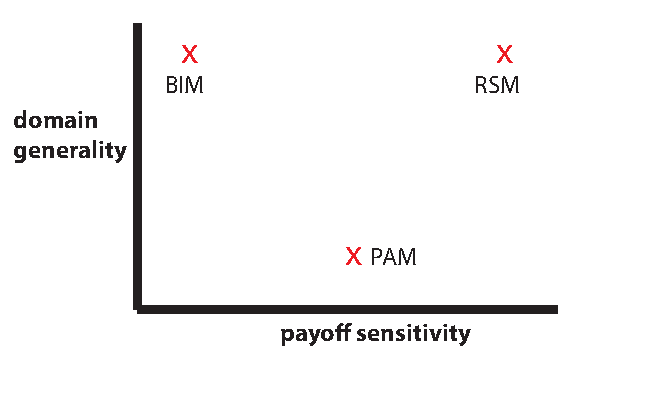
\includegraphics[scale=1]{Fig2}
 \caption{The types of agent (Biased Imitating Mind, Rational Strategising Mind, Pleistocene Adapted Mind) hypothesised to produce cooperative behaviour in societies of any scale. The payoff-sensitivity scale shows the extent to which the decision-making mechanism of the agent is sensitive to expected material payoff. The domain-generality scale shows the extent to which cooperative behaviour is produced by general purpose as opposed to specialised cognitive mechanisms. }
 \end{figure}

\end{document}


 